\documentclass[9pt, xcolor=svgnames]{beamer}
\usepackage[utf8]{inputenc}
\usepackage[T1]{fontenc}
\usepackage[spanish]{babel}

\usetheme[progressbar=frametitle]{metropolis}
\metroset{sectionpage=none, subsectionpage=none}
\usepackage{appendixnumberbeamer}
\usepackage{booktabs}
\usepackage{amsmath, amssymb, bm}
\usepackage{physics}
\usepackage{multicol}
\usepackage{graphicx}
\usepackage{tikz}
\usepackage{minted}
\usemintedstyle{tango}
\setminted{fontsize=\scriptsize, breaklines, linenos, bgcolor=LightGray!20, frame=lines}
\newminted{python}{fontsize=\scriptsize, breaklines, linenos, bgcolor=LightGray!20, frame=lines}
\usepackage{pgfplots}
\pgfplotsset{compat=1.18}
\usepackage{ragged2e}
\usepackage{xspace}
\newcommand{\themename}{\textbf{\textsc{metropolis}}\xspace}

\setbeamercolor{block title}{bg=MidnightBlue!85, fg=white}
\setbeamercolor{block body}{bg=MidnightBlue!5, fg=black}
\setbeamercolor{alerted text}{fg=Crimson}
\setbeamercolor{frametitle}{bg=MidnightBlue!10, fg=black}
\setbeamertemplate{blocks}[rounded][shadow=true]

\title[PCFI261 -- Semana 03]{Modelos Computacionales PCFI261\\Semana 03: Fractales, autosimilitud y dimensión fractal}
\author[Joaquín Peralta]{\large Joaquín Peralta \texttt{<joaquin.peralta@unab.cl>}}
\titlegraphic{\hfill
\includegraphics[height=1.8cm]{logo-unab.jpg}}
\date{Sesión 03 dividida en dos clases de 2 horas}

\begin{document}

\frame{\titlepage}

\begin{frame}{Ruta de la semana}
\begin{columns}[T]
\begin{column}{0.49\textwidth}
\begin{block}{Clase 1}
\begin{itemize}
    \item ¿Qué es un fractal?
    \item Autosimilitud y dimensión.
    \item Ejemplos geométricos y naturales.
    \item Programación: triángulo de Sierpinski y helecho de Barnsley.
\end{itemize}
\end{block}
\end{column}
\begin{column}{0.49\textwidth}
\begin{block}{Clase 2}
\begin{itemize}
    \item Set de Mandelbrot y tiempo de escape.
    \item Conteo de cajas para estimar dimensión fractal.
    \item Función de Weierstrass como ejemplo de rugosidad.
    \item Programación: Mandelbrot y estimación de dimensión.
\end{itemize}
\end{block}
\end{column}
\end{columns}

\vspace{0.4cm}
\begin{alertblock}{Sugerencia de distribución}
En cada clase: \textbf{30--45 min} de teoría + \textbf{75--90 min} de trabajo práctico guiado con Python.
\end{alertblock}
\end{frame}

\section{Clase 1}

\begin{frame}[plain]
\centering
\vfill
{\Huge \bfseries Clase 1}\\[0.4cm]
{\Large Fractales geométricos, autosimilitud y algoritmos iterativos}
\vfill
\end{frame}

\begin{frame}{Objetivos de la Clase 1}
\begin{itemize}
    \item Entender por qué la noción usual de dimensión no siempre es suficiente.
    \item Reconocer la idea de \alert{autosimilitud}: un objeto se parece a sí mismo al cambiar de escala.
    \item Implementar algoritmos iterativos simples para generar fractales.
    \item Relacionar reglas matemáticas muy compactas con patrones visuales complejos.
\end{itemize}
\end{frame}

\begin{frame}{El concepto de dimensión}
\begin{columns}[T]
\begin{column}{0.42\textwidth}
\centering

\includegraphics[width=0.75\linewidth]{triangle.png}\\[0.2cm]
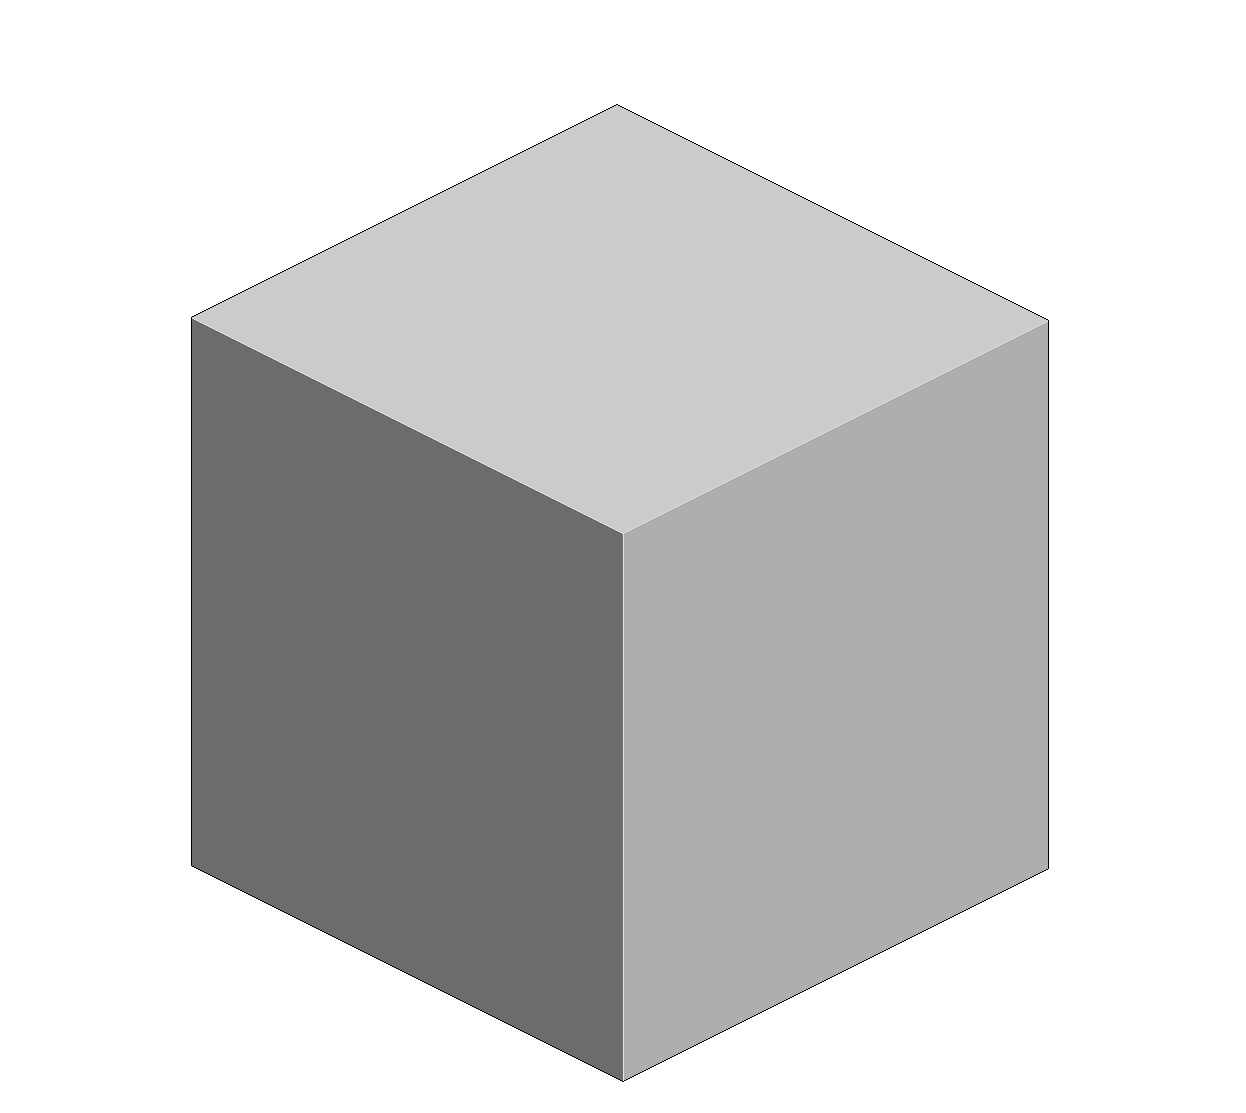
\includegraphics[width=0.75\linewidth]{cube.png}
\end{column}
\begin{column}{0.58\textwidth}
\begin{block}{Escalamiento geométrico}
Si una longitud característica es $L$, entonces de forma muy general
\[
M \propto L^d,
\]
donde $d$ codifica la dimensión efectiva del objeto.
\end{block}

\begin{itemize}
    \item Para un área: $M \propto L^2$.
    \item Para un volumen: $M \propto L^3$.
    \item Para una curva suave: típicamente $M \propto L^1$.
\end{itemize}

La idea fractal aparece cuando el exponente $d$ \textbf{no es entero}.
\end{column}
\end{columns}
\end{frame}

\begin{frame}{La idea de fractal}
\begin{block}{Definición operativa}
Un fractal es un objeto cuya geometría exhibe estructura a múltiples escalas, usualmente con \textbf{autosimilitud} y con una \textbf{dimensión fractal} no entera.
\end{block}

\vspace{0.2cm}
\[
M(L) \propto L^d, \qquad d \in \mathbb{R}.
\]

\begin{itemize}
    \item Si $1<d<2$, el objeto ``llena'' más que una curva, pero menos que una superficie.
    \item Si al hacer zoom siguen apareciendo detalles con estructura parecida, hablamos de autosimilitud.
    \item En computación, los fractales son un gran laboratorio para combinar matemática, iteración y visualización.
\end{itemize}
\end{frame}

\begin{frame}{Fractales en la naturaleza}
\begin{columns}
\begin{column}{0.33\textwidth}
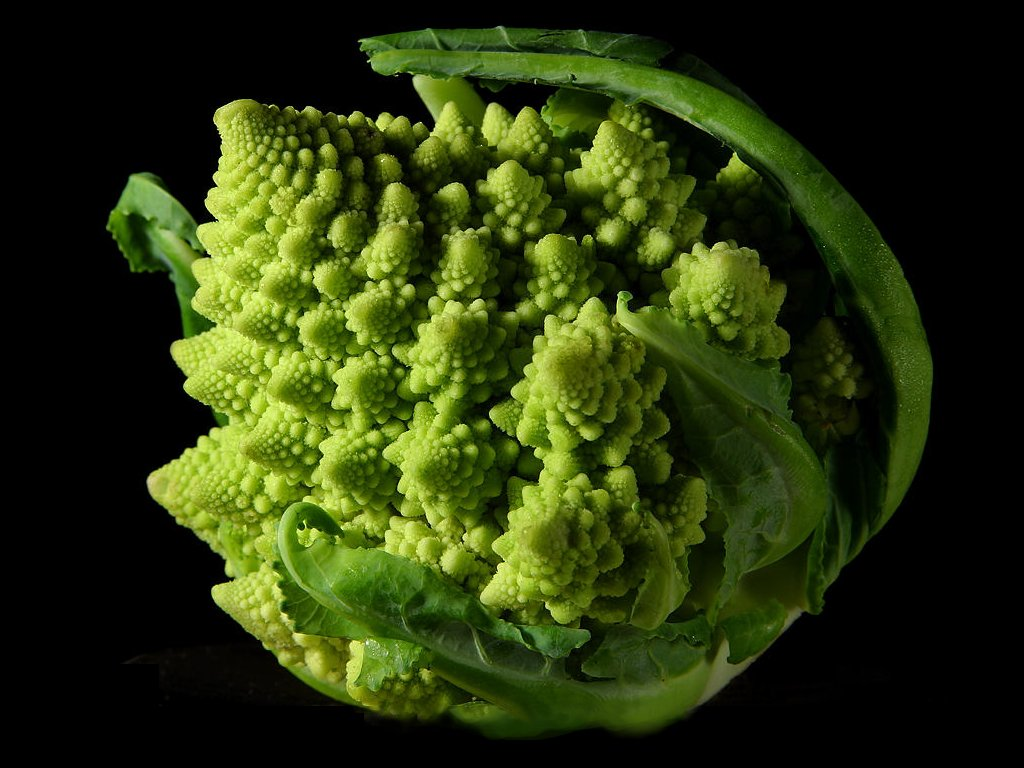
\includegraphics[width=\linewidth]{fractal-broccoli.jpg}
\end{column}
\begin{column}{0.33\textwidth}
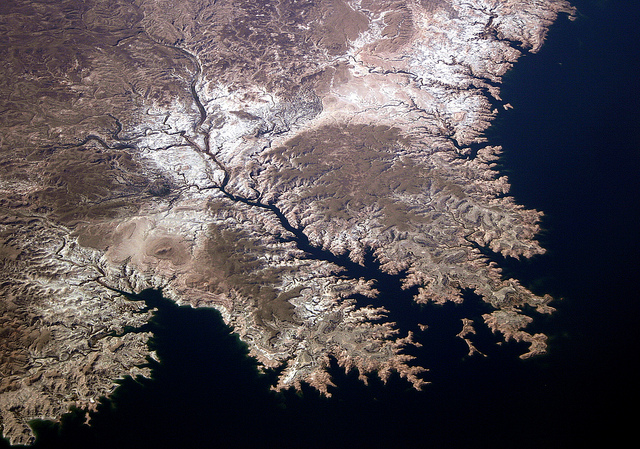
\includegraphics[width=\linewidth]{fractal-coast.jpg}
\end{column}
\begin{column}{0.33\textwidth}
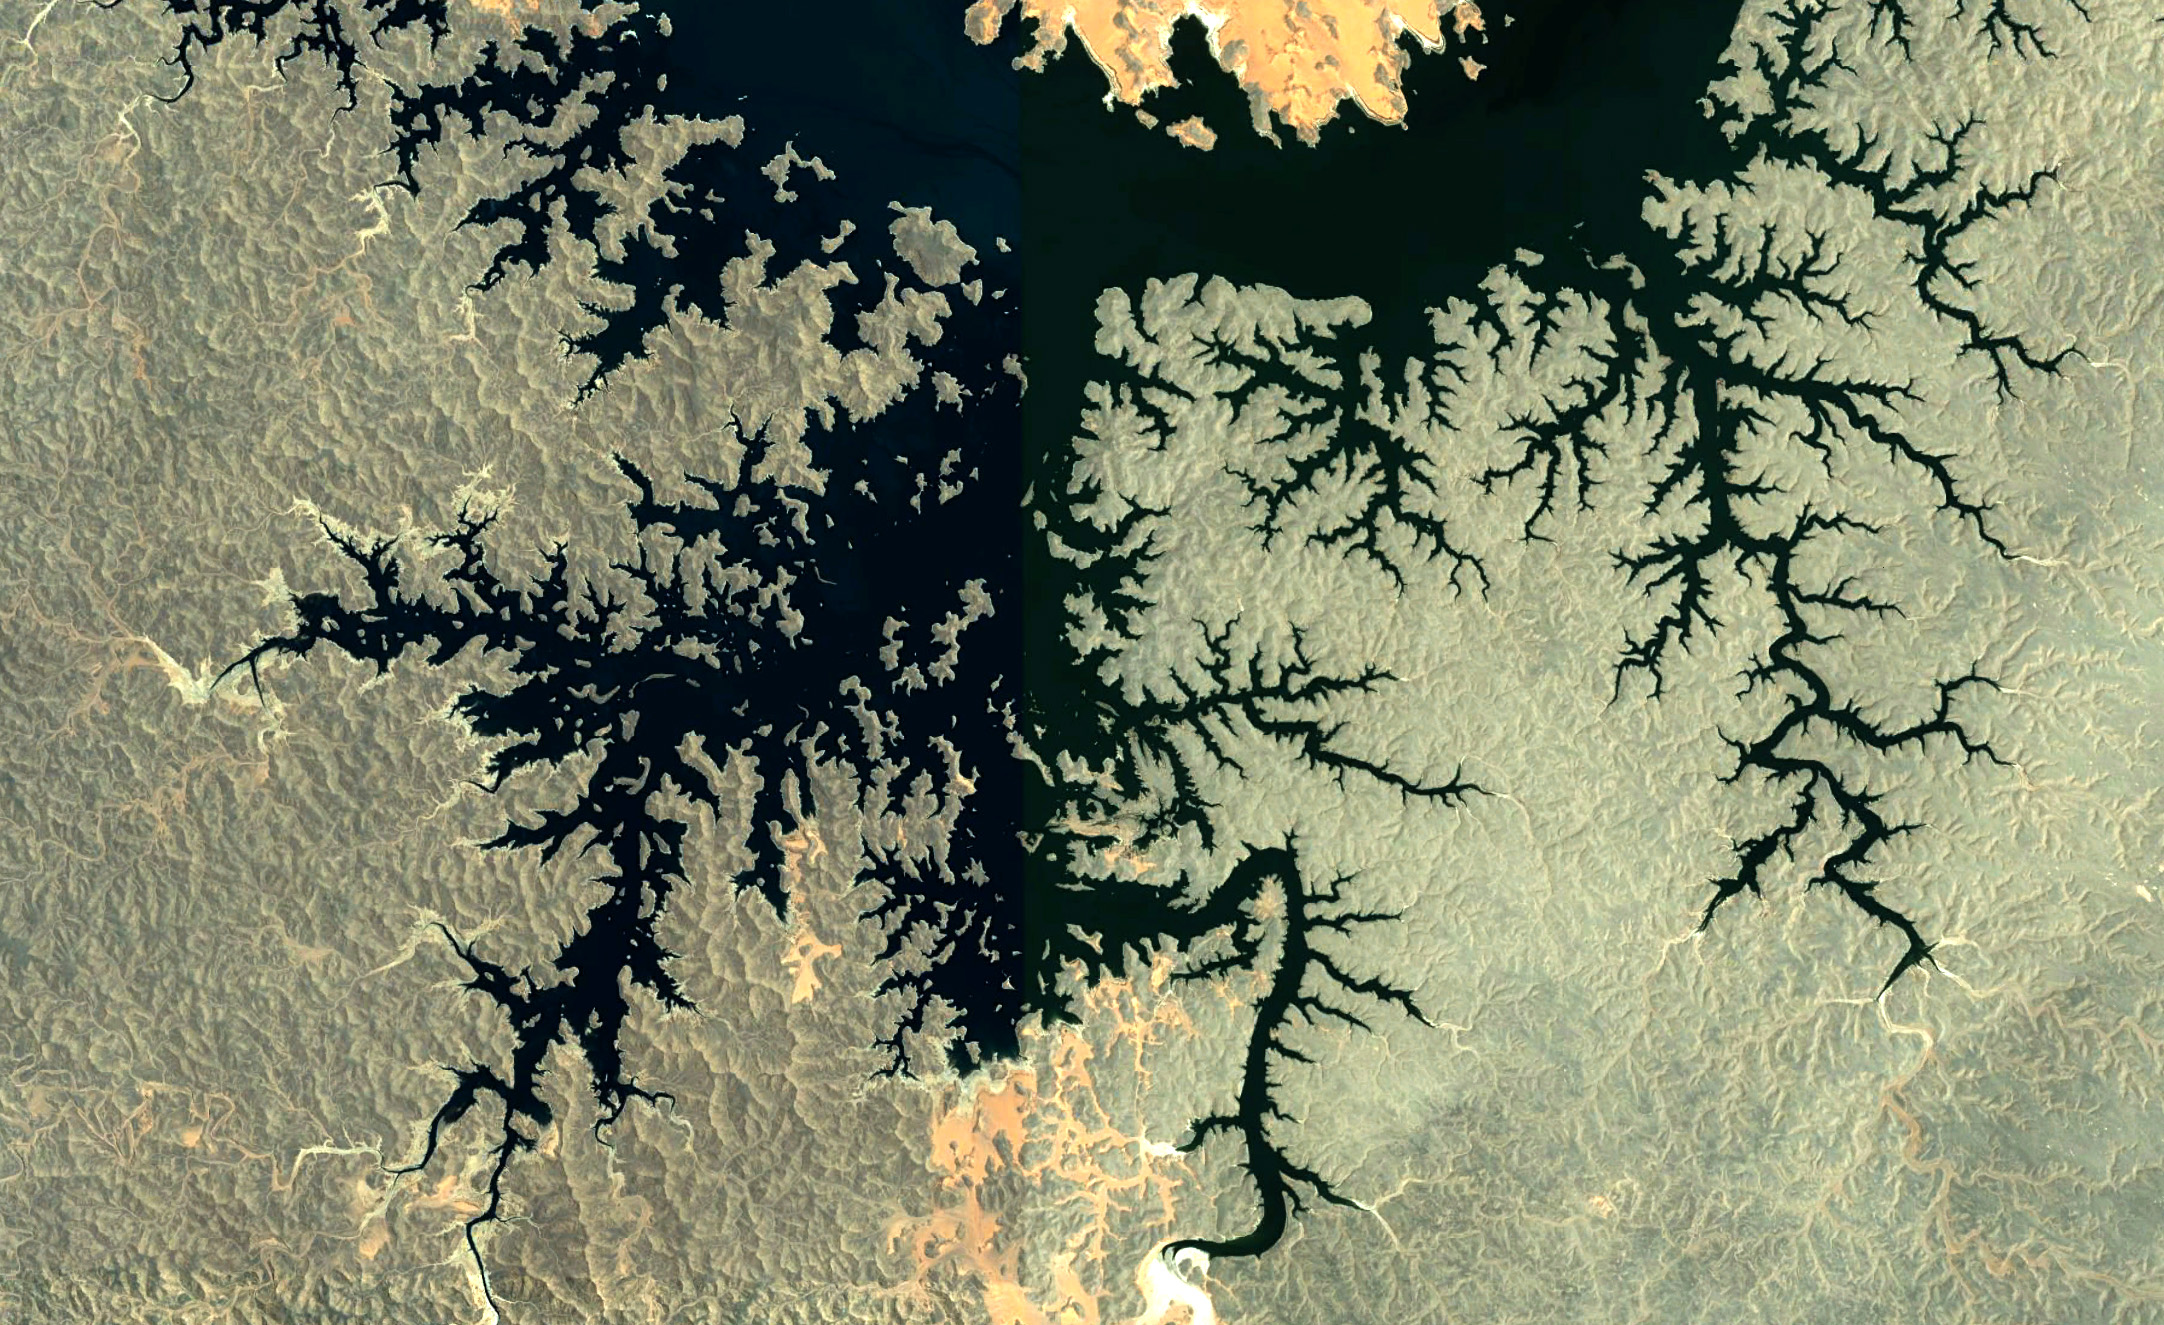
\includegraphics[width=\linewidth]{fractal-photo.jpg}
\end{column}
\end{columns}

\vspace{0.3cm}
\begin{alertblock}{Observación}
Brócoli romanesco, costas, árboles, vasos sanguíneos y muchas superficies rugosas muestran patrones que recuerdan a la autosimilitud fractal, al menos en cierto rango de escalas.
\end{alertblock}
\end{frame}

\begin{frame}{Ejemplo clásico: copo de nieve de Koch}
\begin{columns}[T]
\begin{column}{0.48\textwidth}
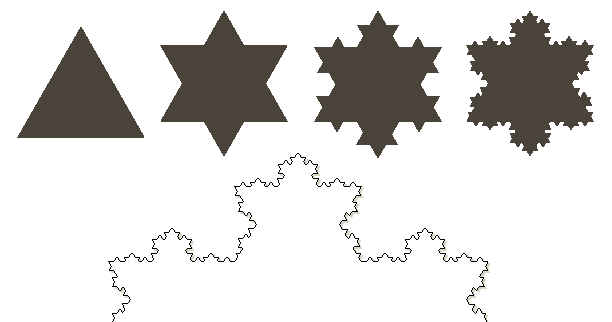
\includegraphics[width=\linewidth]{fractal-snowflake.png}
\end{column}
\begin{column}{0.52\textwidth}
\begin{block}{Construcción}
En cada iteración, cada segmento se reemplaza por cuatro segmentos más pequeños, cada uno de longitud $1/3$ del original.
\end{block}

\[
N = 4, \qquad r = 3
\]
\[
d = \frac{\log N}{\log r} = \frac{\log 4}{\log 3} \approx 1.262
\]

Es uno de los primeros ejemplos donde la dimensión geométrica natural deja de ser un entero.
\end{column}
\end{columns}
\end{frame}

\begin{frame}{Triángulo de Sierpinski}
\begin{columns}
\begin{column}{0.47\textwidth}
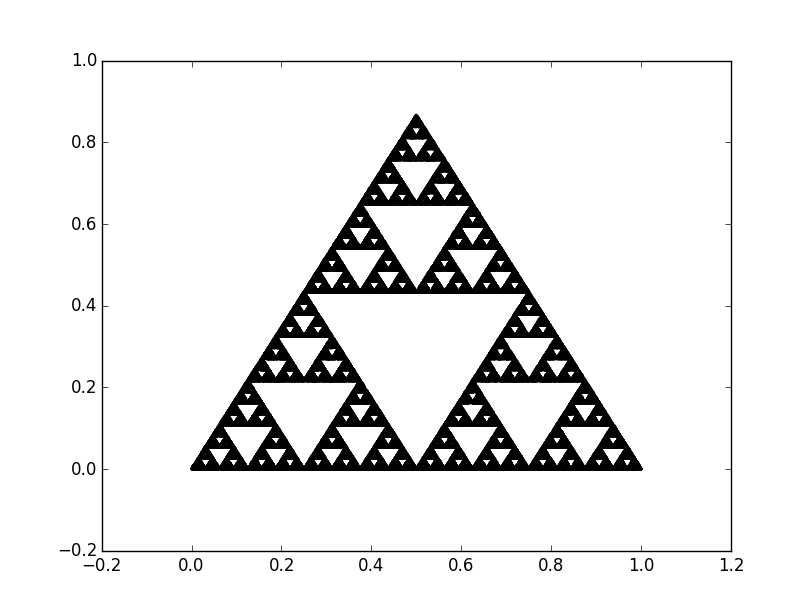
\includegraphics[width=\linewidth]{sierpinski.png}
\end{column}
\begin{column}{0.53\textwidth}
\begin{block}{Idea}
Partimos de un triángulo y aplicamos una regla repetitiva que conserva tres copias reducidas del objeto.
\end{block}

Si cada copia tiene factor de escala $1/2$ y aparecen $3$ copias,
\[
d = \frac{\log 3}{\log 2} \approx 1.585.
\]

Es un ejemplo ideal para introducir algoritmos aleatorios que convergen rápidamente a una estructura fractal.
\end{column}
\end{columns}
\end{frame}

\begin{frame}{Algoritmo estocástico para Sierpinski}
\small
\begin{enumerate}
    \item Defina tres vértices $A_1,A_2,A_3$ de un triángulo equilátero.
    \item Elija un punto inicial $(x_0,y_0)$ dentro del triángulo.
    \item Escoja al azar uno de los tres vértices.
    \item Reemplace el punto por el punto medio entre la posición actual y el vértice elegido:
    \[
    (x_{i+1},y_{i+1}) = \frac{1}{2}(x_i,y_i)+\frac{1}{2}(a_n,b_n).
    \]
    \item Repita miles de veces.
\end{enumerate}

\begin{alertblock}{Idea computacional}
Aunque la regla usa azar, el conjunto límite no es arbitrario: emerge una estructura determinista muy precisa.
\end{alertblock}
\end{frame}

\begin{frame}[fragile]{Código base: triángulo de Sierpinski}
\inputminted[firstline=1,lastline=18]{python}{sierpinski.py}
\end{frame}

\begin{frame}{Helecho de Barnsley}
\begin{columns}
\begin{column}{0.45\textwidth}
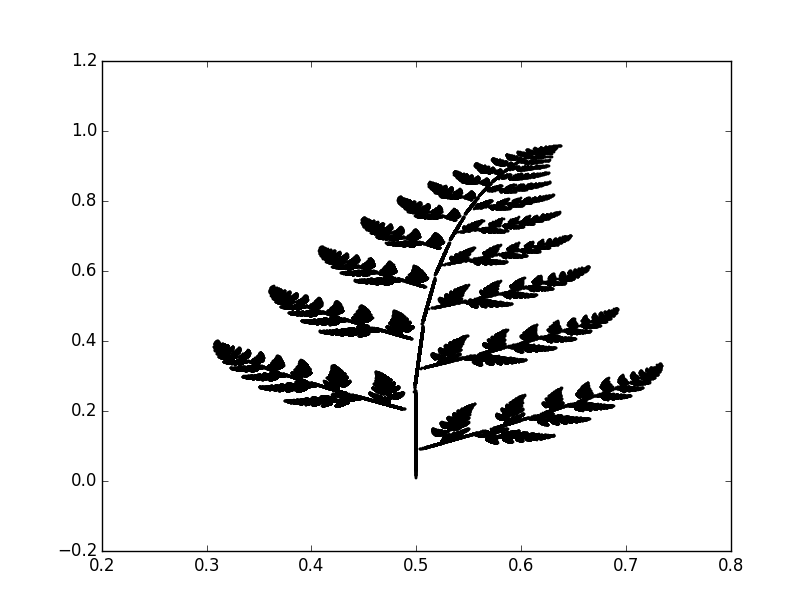
\includegraphics[width=\linewidth]{fern.png}
\end{column}
\begin{column}{0.55\textwidth}
\begin{block}{Transformaciones afines iteradas}
El helecho se genera aplicando varias transformaciones lineales y traslaciones con distintas probabilidades.
\end{block}

Cada regla es de la forma
\[
\bm{r}_{n+1} = A\bm{r}_n + \bm{b},
\]
con una matriz $A$ y un vector $\bm{b}$ distintos según el caso.

Esto introduce la noción de \textbf{sistemas de funciones iteradas} (IFS).
\end{column}
\end{columns}
\end{frame}

\begin{frame}{Algoritmo del helecho de Barnsley}
\small
\begin{itemize}
    \item Partimos desde un punto inicial, por ejemplo $(x,y)=(0.5,0)$.
    \item En cada iteración se elige una transformación según una probabilidad dada.
    \item Algunas reglas generan el tallo, otras las hojas laterales y la estructura principal.
\end{itemize}

\vspace{0.2cm}
\begin{block}{Lección importante}
Un patrón complejo no siempre requiere una ecuación complicada: basta una regla iterativa simple aplicada muchas veces.
\end{block}

\vspace{0.1cm}
\begin{center}
\small La estadística de elección de reglas controla la densidad relativa de distintas regiones del fractal.
\end{center}
\end{frame}

\begin{frame}[fragile]{Código base: helecho de Barnsley}
\inputminted[firstline=1,lastline=21]{python}{fern.py}
\end{frame}

\begin{frame}{Trabajo práctico sugerido -- Clase 1}
\begin{block}{Parte teórica breve (30--45 min)}
Dimensión, autosimilitud, ejemplo de Koch, introducción a IFS y discusión de por qué reglas simples producen patrones complejos.
\end{block}

\begin{block}{Parte de programación (75--90 min)}
\begin{enumerate}
    \item Implementar el triángulo de Sierpinski.
    \item Probar cómo cambia la imagen al variar el número de iteraciones.
    \item Implementar el helecho de Barnsley.
    \item Comparar scatter plots, escalas y colores.
\end{enumerate}
\end{block}

\begin{alertblock}{Desafíos opcionales}
Usar colores por iteración, guardar figuras a archivo y encapsular cada generador en funciones reutilizables.
\end{alertblock}
\end{frame}

\section{Clase 2}

\begin{frame}[plain]
\centering
\vfill
{\Huge \bfseries Clase 2}\\[0.4cm]
{\Large Mandelbrot, tiempo de escape y estimación de dimensión fractal}
\vfill
\end{frame}

\begin{frame}{Objetivos de la Clase 2}
\begin{itemize}
    \item Entender cómo una iteración en el plano complejo genera el set de Mandelbrot.
    \item Introducir el criterio de \alert{tiempo de escape} para construir visualizaciones.
    \item Presentar el método de \alert{box counting} para estimar dimensiones fractales.
    \item Vincular la geometría fractal con funciones rugosas como la de Weierstrass.
\end{itemize}
\end{frame}

\begin{frame}{El set de Mandelbrot}
\begin{columns}
\begin{column}{0.50\textwidth}
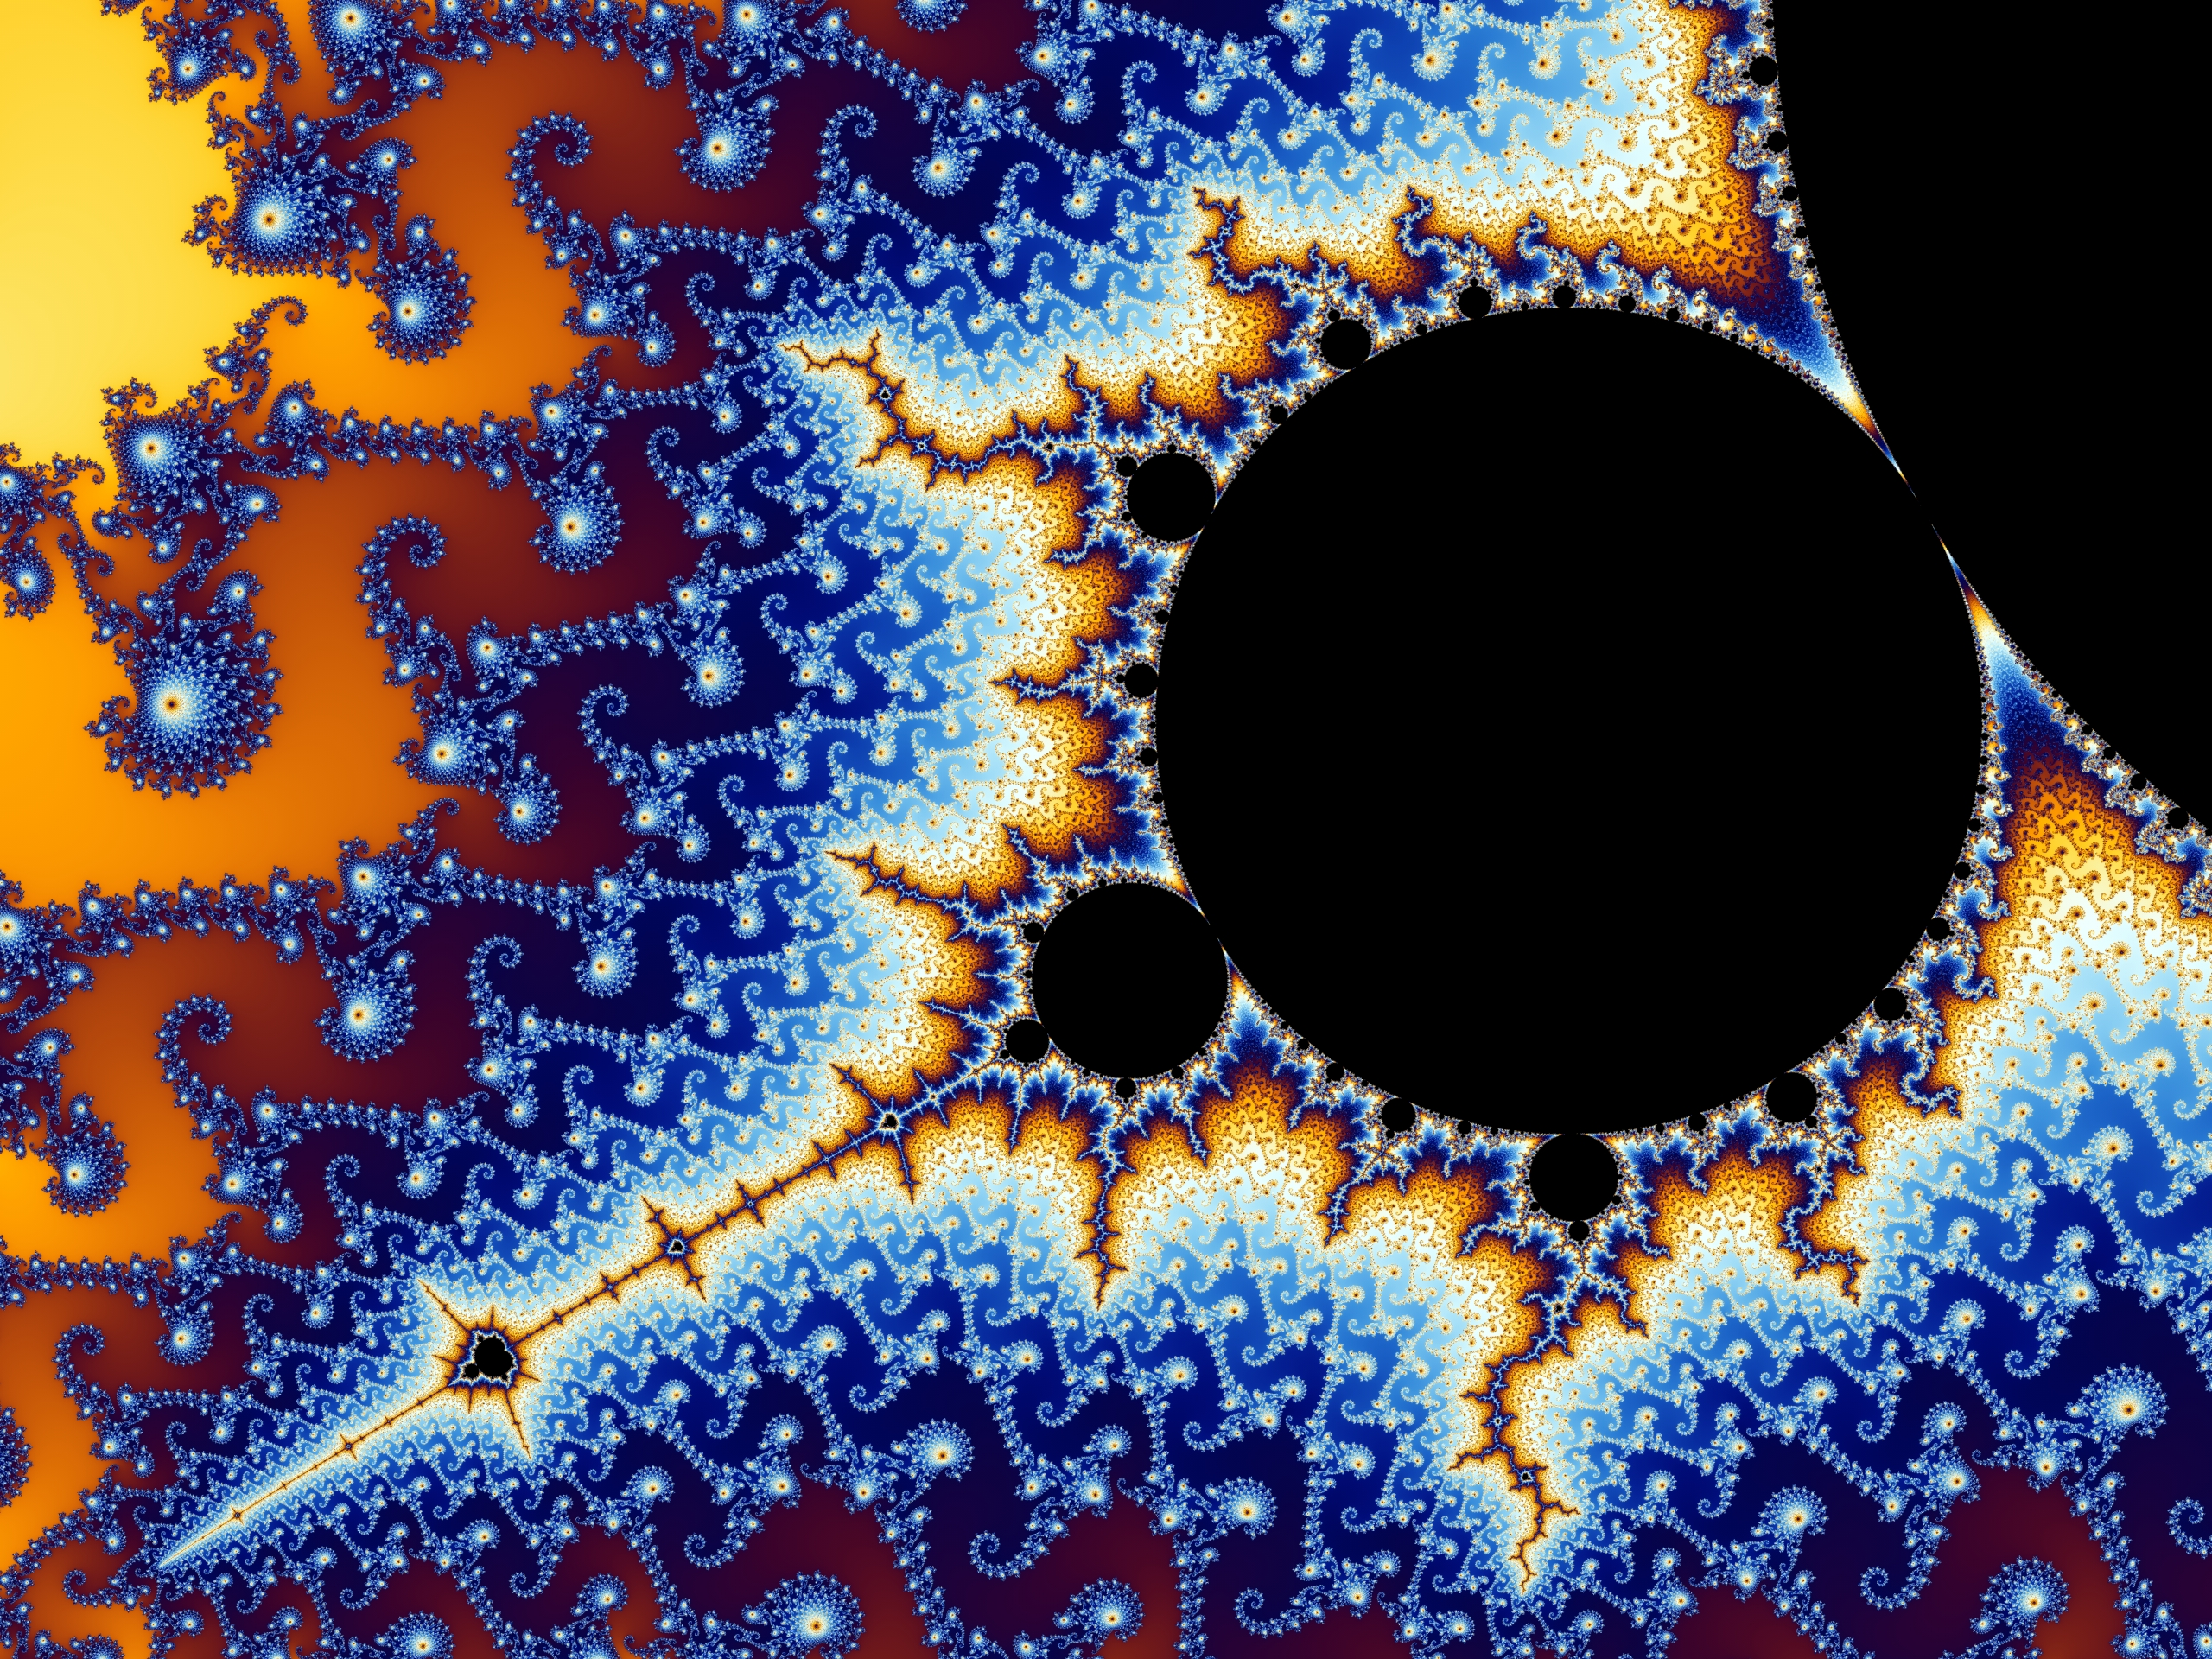
\includegraphics[width=\linewidth]{mandelbrot-wikipedia.jpg}
\end{column}
\begin{column}{0.50\textwidth}
\begin{block}{Definición}
Para cada número complejo $C$, se estudia la órbita generada por
\[
z_{n+1}=z_n^2+C, \qquad z_0=0.
\]
\end{block}

El punto $C$ pertenece al set si la sucesión no escapa hacia infinito.

\vspace{0.15cm}
En la práctica, si en algún momento $|z_n|>2$, sabemos que la órbita escapará.
\end{column}
\end{columns}
\end{frame}

\begin{frame}{Tiempo de escape y coloreado}
\begin{columns}[T]
\begin{column}{0.48\textwidth}
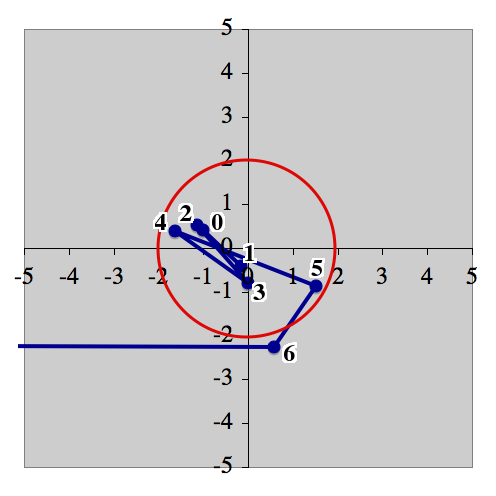
\includegraphics[width=\linewidth]{escapetime.png}
\end{column}
\begin{column}{0.52\textwidth}
\begin{block}{Idea numérica}
Para cada punto $C=x+iy$, contamos cuántas iteraciones tarda la órbita en salir del disco $|z|\le 2$.
\end{block}

\[
T(C)=\min\{n:\ |z_n|>2\}
\]

\begin{itemize}
    \item Si nunca escapa dentro de un máximo $N_{\max}$, se considera interior al set.
    \item Si escapa rápido, el valor de $T$ es pequeño.
    \item $T$ se puede mapear a una paleta de colores.
\end{itemize}
\end{column}
\end{columns}
\end{frame}

\begin{frame}[fragile]{Código base: Mandelbrot binario}
\inputminted[firstline=1,lastline=18]{python}{mandelbrot.py}
\end{frame}

\begin{frame}[fragile]{Código base: Mandelbrot con tiempo de escape}
\inputminted[firstline=1,lastline=18]{python}{mandelbrot2.py}
\end{frame}

\begin{frame}{Resultado con color por tiempo de escape}
\begin{center}
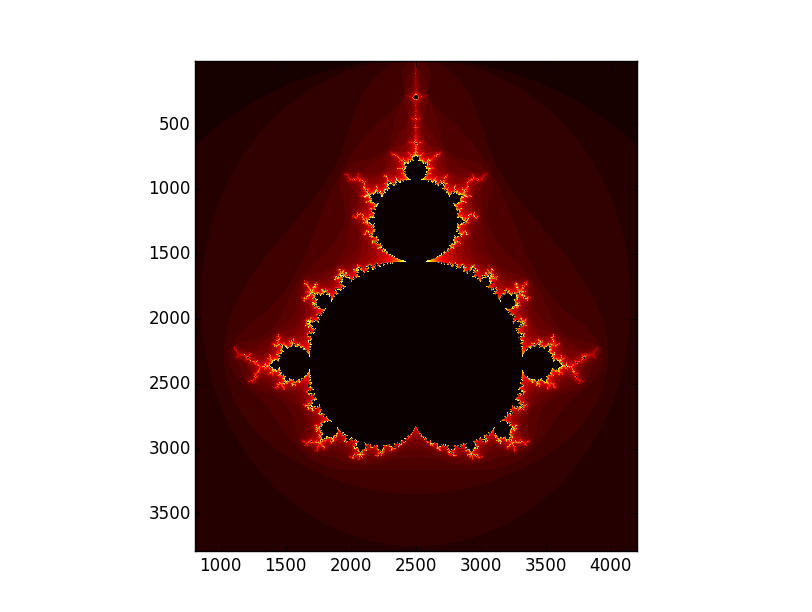
\includegraphics[width=0.82\linewidth]{mandelbrot2.png}
\end{center}
\end{frame}

\begin{frame}{Dimensión fractal y box counting}
\begin{columns}
\begin{column}{0.46\textwidth}
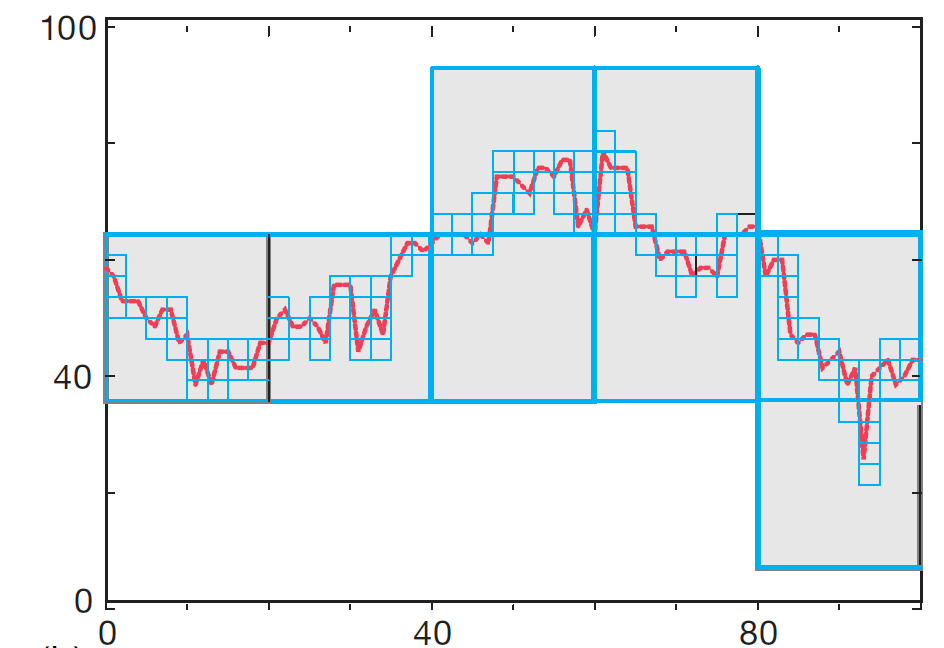
\includegraphics[width=\linewidth]{boxcounting.png}
\end{column}
\begin{column}{0.54\textwidth}
\begin{block}{Método}
Cubra el objeto con una grilla de $N\times N$ cajas y cuente cuántas cajas, $U(N)$, contienen parte del conjunto.
\end{block}

Si el objeto es fractal,
\[
U(N) \sim U_0 N^d.
\]
Tomando logaritmos,
\[
\log U(N)=\log U_0 + d\log N.
\]

Así, la pendiente en un gráfico log-log estima la dimensión fractal $d$.
\end{column}
\end{columns}
\end{frame}

\begin{frame}{Cómo implementar box counting en Python}
\small
\begin{enumerate}
    \item Generar o cargar un conjunto de puntos $(x_i,y_i)$.
    \item Elegir varios tamaños de grilla: $N=8,16,32,64,\dots$.
    \item Convertir cada punto al índice de caja correspondiente.
    \item Contar cuántas cajas distintas quedan ocupadas.
    \item Ajustar una recta en el gráfico $(\log N,\log U)$.
\end{enumerate}

\begin{alertblock}{Interpretación}
Para un disco lleno en 2D esperamos $d\approx 2$; para una curva suave, $d\approx 1$; para un fractal, un valor intermedio o no entero.
\end{alertblock}
\end{frame}

\begin{frame}{La función de Weierstrass}
\begin{columns}
\begin{column}{0.45\textwidth}
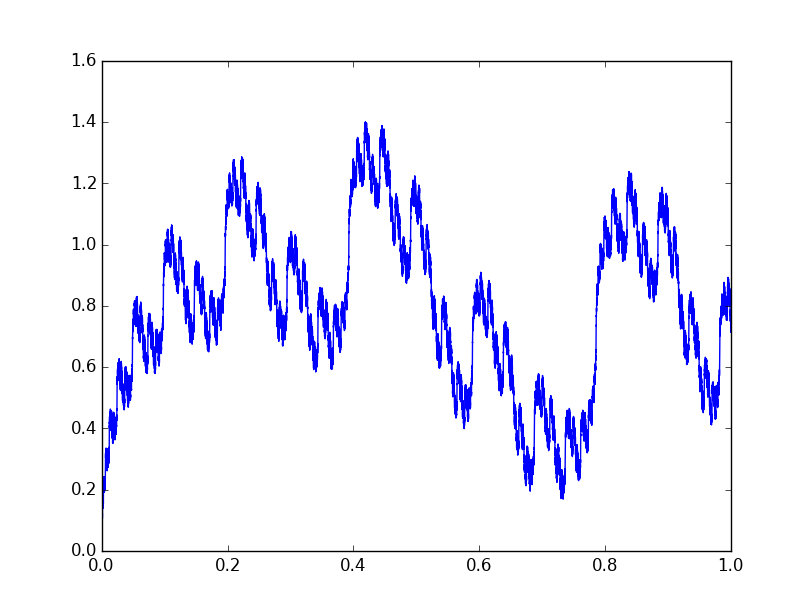
\includegraphics[width=\linewidth]{weierstrass.png}
\end{column}
\begin{column}{0.55\textwidth}
\begin{block}{Ejemplo de rugosidad extrema}
Una versión típica es
\[
f(x)=\sum_{k=1}^{\infty} \frac{\sin(2^k x)}{(\sqrt{2})^k}.
\]
\end{block}

Es continua en todos los puntos, pero no diferenciable en ninguno.\newline
Su gráfica mantiene irregularidad a toda escala, lo que la vuelve un ejemplo natural para explorar métodos numéricos de dimensión.
\end{column}
\end{columns}
\end{frame}

\begin{frame}{Trabajo práctico sugerido -- Clase 2}
\begin{block}{Parte teórica breve (30--45 min)}
Iteración compleja, criterio de escape, visualización por colores y método de conteo de cajas con ajuste log-log.
\end{block}

\begin{block}{Parte de programación (75--90 min)}
\begin{enumerate}
    \item Generar el set de Mandelbrot binario.
    \item Extenderlo a tiempo de escape y coloreado.
    \item Estimar por box counting la dimensión de un disco lleno.
    \item Repetir la estimación para el helecho de Barnsley o la gráfica de Weierstrass.
\end{enumerate}
\end{block}
\end{frame}

\begin{frame}{Actividades integradas de la semana}
\begin{enumerate}
    \item[(a)] Genere el triángulo de Sierpinski usando el algoritmo estocástico.
    \item[(b)] Genere el helecho de Barnsley usando el algoritmo estocástico.
    \item[(c)] Genere el set de Mandelbrot coloreando por tiempo de escape.
    \item[(d)] Estime la dimensión de un círculo lleno mediante conteo de cajas.
    \item[(e)] Estime la dimensión fractal del helecho de Barnsley o de la función de Weierstrass.
\end{enumerate}

\vspace{0.25cm}
\begin{alertblock}{Entrega sugerida}
Pedir al estudiantado un notebook o script con: código, figuras generadas y una breve interpretación del valor estimado de $d$.
\end{alertblock}
\end{frame}

\begin{frame}{Resumen}
\begin{itemize}
    \item Los fractales combinan iteración, geometría y visualización computacional.
    \item La dimensión fractal cuantifica cuánto ``llena'' el espacio un objeto irregular.
    \item Sierpinski, Barnsley y Mandelbrot muestran tres mecanismos distintos: reglas geométricas, IFS y dinámica compleja.
    \item El método de conteo de cajas permite pasar de la imagen a una estimación cuantitativa.
\end{itemize}
\end{frame}

\end{document}
